\section{Incentivization Mechanism}
\label{sec:incentiviationmechanism}

The HOPR protocol provides incentives to nodes in the network to achieve correct transformation and delivery of mixnet packets. This is accomplished through a combination of \lcnameref{sec:proofofrelay}, a novel mechanism which is cost effective and privacy preserving, and \lcnameref{sec:probabilisticpayments}, together with an on-chain \lcnameref{sec:onchaincommitment}. The high-level overview of the motivation behind this incentive scheme was covered in the \lcnameref{sec:introduction}. This section focuses on the technical details used to implement the mechanism.

\paragraph{Construction}

\begin{itemize}
    \item Every packet is sent together with a ticket.
    \item Each ticket contains a challenge.
    \item The validity of a ticket can be checked on reception of the packet but the on-chain logic enforces a solution to the challenge stated in the ticket.
    \item The challenge can be solved \textit{after} the packet has been forwarded.
\end{itemize}

\subsection{Proof of Relay}
\label{sec:proofofrelay}

HOPR incentivizes packet transformation and delivery using a mechanism called \textbf{proof of relay}. This mechanism guarantees that a node's relay services are verifiable.

\paragraph{Secret sharing}
\label{sec:proofofrelay:secretSharing}

Each node derives two keys, $s_i^{own}$ and $_i^{ack}$, by using the $s_i$ as given by the SPHINX packet, see section \lcnameref{appendix:keyderivation} for more details. $s_i^{own}$ and $s_{i+1}^{ack}$ serve as key shares of a 2-out-of-2 secret sharing between a node $n_i$ and the next downstream node $n_{i+1}$ along the chosen path. Once a node knows \textit{both} key shares, $s_i^{own}$ and $s_{i+1}^{ack}$, it is able to reconstruct $s_i^{response}$ to redeem the received ticket on-chain.

Whilst $s_i^{own}$ is derivable upon reception of a packet, $s_{i+1}^{ack}$ requires the cooperation of the next downstream node $n_{i+1}$ and is sent as an \textit{acknowledgement} if $n_{i+1}$ has received the transformed packet \textit{and} considers packet as well as the embedded ticket valid.

\begin{figure}[H]
    \centering
    \begin{tikzpicture}[auto]
        \draw (0,0) node (a) {};
        \draw (3.0,0) node (b) [rectangle,draw] {$n_{i-1}$};
        \draw (6,0) node (c) [rectangle,draw] {$n_i$};
        \draw (9.0,0) node (d) [rectangle,draw] {$n_{i+1}$};
        \draw (12.0,0) node (e) {};

        \draw (6.0, -1.5) node [circle,draw] (intermediateResult) {};
        \draw (6.0, -2.5) node (response) {$s_i^{response}$};

        \draw [->,draw,dashed] (a.east) to node [align=center,below] {packet$_{i-2}$} (b.west);
        \draw [->,draw,dashed] (b.east) to node [align=center,below] {packet$_{i-1}$} node [align=center,above,circle] {\color{hopr-blue}1.} (c.west);
        \draw [->,draw,dashed] (c.east) to node [align=center,below] {packet$_i$} node [align=center,above,circle] {\color{hopr-blue}2.} (d.west);
        \draw [->,draw,dashed] (d.east) to node [align=center,below] {packet$_{i+1}$} (e.west);

        \draw [->,draw] (c.south) to node [right] {$s_i^{own}$} node [align=center,left=1pt,circle] {\color{hopr-blue}3.}  (intermediateResult.north);
        \draw [->,draw,bend left] (d.south) to node[below] {$s_{i+1}^{ack}$} node [align=center,right=5pt,circle] {\color{hopr-blue}4.} (intermediateResult.east);
        \draw [->,draw] (intermediateResult.south) to (response.north);
    \end{tikzpicture}
    \caption{\color{hopr-blue}1. \color{black} Node $n_i$ receives $packet_{i-1}$, validates it, transforms it and \color{hopr-blue}2. \color{black} sends it to node $n_{i+1}$. \color{hopr-blue}3. \color{black} While processing $packet_i$, node $n_i$ derives $s_i^{own}$ and once node $n_{i+1}$ considered $packet_i$ valid, it \textit{acknowledges} the reception of $packet_i$ and thereby reveals $s_{i+1}^{ack}$ to node $n_i$ which allows node $n_i$ to reconstruct $s_i^{response}$.}
    \label{fig:proofofrelay}
\end{figure}

\paragraph{Challenge-response}

Tickets that that are sent next to a mixnet packet include a challenge $C_i$ which is computed as $$C_i = s_i^{response} \cdot G = (s_i^{own} + s_{i+1}^{ack}) \cdot G$$ where $G$ refers to the base-point and $\cdot$ means scalar multiplication on the curve. Hence, in order to solve the challenge, it is necessary to know $s_i^{own}$ as well as $s_{i+1}^{ack}$.

\paragraph{Challenge and Hint}
\label{sec:proofofrelay:challenge}

Once a node receives a packet, it is able to derive $s_i^{own}$ but it is unable to decide whether $s_{i+i}^{ack}$ will ever lead to $s_i^{response}$ that solves the challenge. Since the underlying field preserves the distributivity, it holds that $$C_i = s_i^{response} \cdot G = (s_i^{own} + s_{i+1}^{ack}) \cdot G = s_i^{own} \cdot G + s_{i+1}^{ack} \cdot G$$

Hence by knowing $hint_i = s_{i+1}^{ack} \cdot G$, the node can verify that $s_i^{own} \cdot G + hint_i = C_i$ and thereby check that the creator of the challenge must have known a value $\tilde{s}_{i+1}^{ack}$ that led to $hint_i$. Due to the infeasibility to invert scalar multiplication on the utilized curve, knwowing $hint_i$ does not reveal $s_{i+1}^{ack}$. Hence, by embedding $hint_i$ into the part of $\beta$ within the SPHINX packet that is readable by node $n_i$, the sender of the makes the validity of the embedded challenge verifiable.

As the next downstream node would not accept a packet without a ticket\footnote{By default, nodes are only forwarding packets that include incentives. Nevertheless, the protocol does not prevent them from processing packets without enforcing an incentive.}, the node $n_i$ does not only need to transform the packet but also issue a ticket to the next downstream node $n_{i+1}$. Therefore, it needs to know \textit{which} challenge $\tilde{C}_{i+1}$ to put into the ticket issued for node $n_{i+1}$. As in the previous section, this is done with the help of the creator of the packet which embeds $C_{i+1}$ into the part of the SPINX packet that is readable by node $n_{i+1}$.

\begin{figure}[H]
    \centering
    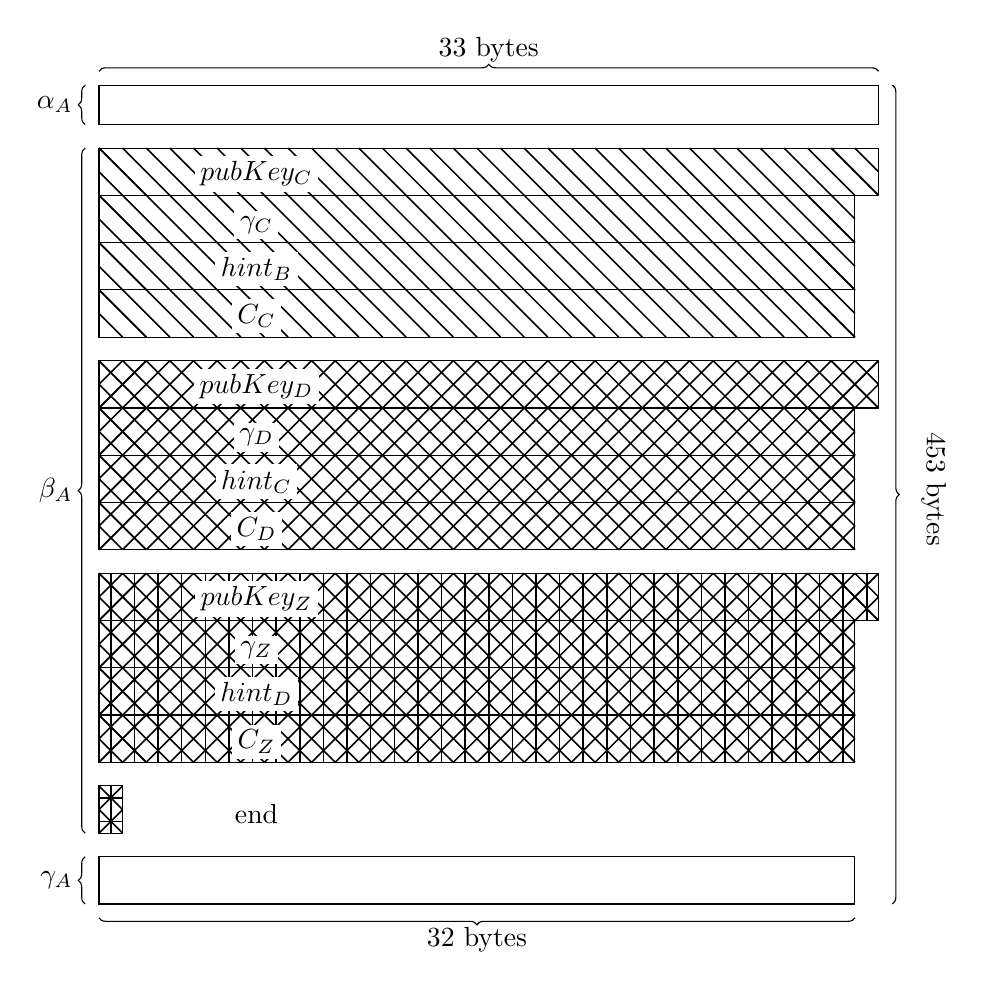
\begin{tikzpicture}
        \def\one{0.3}
        \draw[decoration={brace,raise=5pt},decorate] (0,0.5) -- node[above=5pt] {33 bytes} (33*\one,0.5);
        \draw[decoration={brace,raise=5pt},decorate] (0,0) -- node[left=6pt] {$\alpha_A$} (0,0.5) ;
        \draw[black] (0,0) rectangle (\one*33,0.5);

        \draw[decoration={brace,raise=5pt},decorate] (0,-9.0) -- node[left=6pt] {$\beta_A$} (0,-0.3);

        \foreach \name\length\offset\hatching in{$pubKey_C$/33/-0.9/1,$\gamma_C$/32/-1.5/1,$hint_B$/32/-2.1/1,$C_C$/32/-2.7/1,$pubKey_D$/33/-3.6/2,$\gamma_D$/32/-4.2/2,$hint_C$/32/-4.8/2,$C_D$/32/-5.4/2,$pubKey_Z$/33/-6.3/3,$\gamma_Z$/32/-6.9/3,$hint_D$/32/-7.5/3,$C_Z$/32/-8.1/3}{
                \draw (0,\offset) rectangle (\one*\length,\offset+0.6);
                \begin{scope}[shift={(0,\offset)}]
                    \ifnum\length=33
                        \def\a{9.9}
                        \def\diff{9.4}
                    \else
                        \def\a{9.6}
                        \def\diff{9.1}
                    \fi
                    \def\b{0.6}
                    \def\lw{0.2}

                    \foreach \x [count=\i] in{0,0.3,0.6,...,\b}{
                            \draw [line width=\lw mm](\x,0)--(0,\x) (\a-\b+\x,\b)--(\a,\x);
                        }
                    \foreach \x [count=\i] in{0,0.3,0.6,...,\diff}{
                            \draw [line width=\lw mm](\x+\b,0)--(\x,\b);
                        }

                    \ifnum\hatching>1
                        \foreach \x [count=\i] in{0,0.3,0.6,...,\b}{
                                \draw [line width=\lw mm](0,\x)--(\b-\x,\b) (\a-\b+\x,0)--(\a,\b-\x);
                            }
                        \foreach \x [count=\i] in{0,0.3,0.6,...,\diff}{
                                \draw [line width=\lw mm](\x,0)--(\b+\x,\b);
                            }
                    \fi

                    \ifnum\hatching>2
                        \foreach \x [count=\i] in{0,0.15,0.45,...,\a}{
                                \draw [line width=\lw mm](\x,0)--(\x,\b);
                            }
                    \fi
                \end{scope}

                \draw (2.0,\offset+0.25) node[fill=white,above=-6pt,inner sep=2pt] {\name};
            }

        \draw (0,-8.4) rectangle (\one*1,-9.0);

        \begin{scope}[shift={(0,-9.0)}]
            \def\lw{0.2}

            \draw [line width=\lw mm](0,0)--(0.3,0.3);
            \draw [line width=\lw mm](0,0.3)--(0.3,0.6);

            \draw [line width=\lw mm](0,0.6)--(0.3,0.3);
            \draw [line width=\lw mm](0,0.3)--(0.3,0);

            \draw [line width=\lw mm](0.15,0)--(0.15,0.6);

            \draw [line width=\lw mm](0,0.15)--(0.3,0.15);
            \draw [line width=\lw mm](0,0.45)--(0.3,0.45);

            \draw (2.0,0.25) node[fill=white,above=-7pt] {end};
        \end{scope}

        \draw[decoration={brace,raise=5pt},decorate] (0,-9.9) -- node[left=6pt] {$\gamma_A$} (0,-9.3);

        \draw (0,-9.3) rectangle (\one*32,-9.9);
        \draw[decoration={brace,mirror,raise=5pt},decorate] (0,-9.9) -- node[below=5pt] {32 bytes} (32*\one,-9.9);

        \draw[decoration={brace,raise=5pt},decorate] (33*\one,0.5) -- node[right=12pt,above=2pt,rotate=-90] {453 bytes} (33*\one,-9.9) ;

    \end{tikzpicture}
    \caption{Mixnet packet header with PoR fields that is sent from the sender $A$ to $B$ and supposed to be forwarded through nodes $C, D$ to $Z$.}
\end{figure}

By chaining this principle, nodes are forced to \textit{always} issue a ticket to the next downstream node because they are unable to claim their own incentive without the help of the next downstream node.

Since the very last node, namely the final receiver, of the packet, does not need to forward the packet to anyone else, it has no direct incentive to acknowledge tickets, hence there are no \textit{direct} consequences for \textit{not} acknowledging packet. In its current version, the protocol does not prevent this kind of behavior but it is foreseen to solve this issue by using a reputation system.

\subsection{On-chain Commitment}
\label{sec:onchaincommitment}

HOPR uses a commitment scheme to deposit values on-chain and reveal them once a
node redeems an incentive for relaying packets. This comes with the benefit that
the redeeming party must disclose a secret that is unknown to the issuer of the
incentive until it is claimed on-chain. The $\textbf{opening}$ $\mathsf{Open}$
and the $\textbf{response}$ $r$ to the proof-of-relay challenge (called \textit{nextCommitment} and \textit{proofOfRelaySecret} in the smart contract) are then
used to prove to the smart contract that the node has a legitimate claim to the
funds. 
HOPR uses a computationally hiding and binding commitment scheme:

\begin{defnsub}
    % Currently leaving out further details such as unconditionally/computationally binding / hiding
    A commitment scheme $\mathsf{C_m} = (\mathsf{Commit}, \mathsf{Open})$ is a protocol between two parties, $A$ and $B$, that gives $A$ the opportunity to store a value $comm = \mathsf{Commit}(x)$ at $B$. The value $x$ stays unknown to $B$ until $A$ decides to reveal it to $B$.
    For any $m\in \mathbb{M}$, $(c,d)\leftarrow \mathsf{Commit(m)}$ is the commitment/opening pair for $m$ where $c = c(m)$ serves as the commitment value, and $d = d(m)$ as the opening value.
    
 \noindent\textbf{Hiding:} A commitment scheme is called \textbf{computationally hiding} if the following holds:
    $$\forall \;x\neq x' \; \{\mathsf{Commit}_k(x,U_k)\}_{k\in\mathbb{N}}\approx\{{\mathsf{Commit}_k(x',U_k)}\}_{k\in\mathbb{N}}.$$ This means both probability ensembles are computationally indistinguishable, such that $U_{k}$ is the uniform distribution over the $2^{k}$ opening values for the security parameter $k$.
    
\noindent\textbf{Binding:} A commitment scheme is called \textbf{computationally binding} if for all bounded polynomial adversary \textit{Adv} algorithms that run in time $t$ with output $x,x',open,open'$, the following holds:
    $$P	[ \,x\neq x' \; and \; \mathsf{Commit}(x,open)={\mathsf{Commit}(x',open')}] \,\leq \epsilon$$ A computationally bounded adversary has limitations on their computational resources. 

\end{defnsub}

\subsubsection{Commitment phase}

Once a node is the destination of a HOPR unidirectional channel, it derives a
master key $comm_0$ from its private key and uses it to create an iterated
commitment $comm_i$ such that for every $i \in \mathbb{N}_0$ and $i > 0$ it
holds that $$ \mathsf{Open}(comm_{i}, comm_{i-1}) = \top,$$ which means opening
$comm_{i}$ with $comm_{i-1}$ holds true.
The iterated commitment is computed as $$comm_n = h^n(comm_0),$$ where $h$ is a
pre-image resistant hash function (we use the keccak256 hash function, which is also used
in Ethereum) and $comm_0$ is derived as $$ comm_0 = \mathsf{h}(privKey,chainId,
contractAddr, channelId, channelEpoch)$$
This will be implemented in the future after further research
determines whether such a design leaks information about the
private key or not. 
The master key should be pseudorandom, such that
all intermediate commitments $comm_{i}$ for $i \in \mathbb{N}_0$ and $0 < i \le
n$ are indistinguishable for the ticket issuer from random numbers of the same
length. This is necessary to ensure that the ticket issuer is unable to
determine whether a ticket is a winner or not when issuing the ticket. This makes
it infeasible for the ticket issuer to tweak the challenge to such that it
cannot be a winner.

When dispatching a transaction that opens the payment channel, the
commitment $comm_n$ is stored in the channel structure in the smart contract and
the smart contract will force the ticket recipient to reveal $comm_{n-1}$ when
redeeming a ticket issued in this channel. The number of iterations $n$ can be
chosen as a constant and should reflect the number of tickets a node intends to
redeem within a channel.

\subsubsection{Opening phase}

In order to redeem a ticket, a node must reveal the opening to the current
commitment $comm_i$ that is stored in the smart contract for the channel. Since
the opening $comm_{i-1}$ allows the ticket issuer to determine whether a ticket
is going to be a winner, the ticket recipient should keep $comm_{i-1}$ until it is
used to redeem a ticket. Tickets lead to a win if: $$\mathsf{h}( t_h, r_i,
comm_{i-1} ) < P_w,$$ where $P_w$ is the ticket's winning probability and
$$t_h=\mathsf{h}(t) \;and\; \mathsf{Open}(comm_i, comm_{i-1}) = \top.$$ Since
$comm_{0}$ is known to the ticket recipient, the ticket recipient can compute
the opening as $comm_{n-1} = \mathsf{h}^{n-1}(comm_0)$. On redeeming a ticket,
the smart contract verifies that $$\mathsf{Open}(comm_i, comm_{i-1}) = \top$$
and sets $channel.comm[redeemer] \leftarrow comm_{i-1}$. Thus the next time the
node redeems a ticket, it must reveal $comm_{i-2}$. In addition, each node is
granted the right to reset the commitment to a new value. This is particularly necessary
once a node reveals $comm_0$ and therefore is with high probability
unable to compute a value $r$ such that $$\mathsf{Open}(comm_0,r) \neq \bot,$$
where $\bot$ represents the truth value ``false". 
Since this mechanism can
be abused by the ticket recipient to tweak the entropy used to determine
whether a ticket is a winner or not, the smart contract keeps track of resets of
the on-chain commitment and sets $$channel[redeemer].ticketEpoch \leftarrow
channel[redeemer].ticketEpoch +1 ,$$ thereby invalidating all previously
unredeemed tickets.


\subsection{Probabilistic Payments}
\label{sec:probabilisticpayments}

In traditional payment channels, two parties $A$ and $B$ lock some funds within a smart contract, make transactions off-chain and only commit the aggregation on-chain. Thus, a payment channel is bidirectional, which means both $A$ and $B$ can send and receive transactions within the same payment channel. The HOPR protocol uses unidirectional payment channels to implement bidirectional payment channel behaviour, where one payment channel is created from $A$ to $B$ and another from $B$ to $A$. The payment channel creator is the sole owner of funds in the payment channel and the only one able to create \textbf{tickets}, encapsulated funds which are described in detail in Section \ref{sec:tickets}. A payment channel created from party $A$ to party $B$ is different from a payment channel created from party $B$ to party $A$.

$$A\rightarrow B \neq B\rightarrow A$$

This separation reflects the directional nature of packets flowing through the network. It also brings the advantage that each payment channel's logic is easier to verify.

\paragraph{Acknowledgements} are messages which allow every node to acknowledge the processing of a packet to the previous node. This acknowledgement ($ACK$) contains the cryptographic material needed to unlock the possible payout for the previous node. Note that an acknowledgement is always sent to the previous node, and using acknowledgments with vanilla payment channels results in accumulated incentives, where the latest acknowledgement contains all previous incentives plus the incentive for the most recent interaction, as explained below:

\begin{align}
value (ACK_n) &=\sum_{i=1}^nfee_{packet_i},
\end{align}
where $n$ is the total number of mixnet packets transformed.

An issue arises when $B$ receives $ACK_n$ for $packet_n$ before sending $packet_{n-1}$. At this point $B$ would have no incentive to process $packet_{n-1}$ rather than $packet_{n}$. To avoid such false incentives, the HOPR protocol utilizes probabilistic payments. A \textit{ticket} can be either a win or a loss, determined based on some winning probability lower than 1. This means nodes are incentivized to continue relaying packets, as they do not know which tickets will result in a payout. From a node's perspective, each ticket has the same value until it is claimed; therefore, the HOPR protocol encourages nodes to claim tickets independently from each other.

\begin{align}
value ( ACK_i )  &  =value ( ACK_j ) \quad for \quad i,j\in \{1,n\}
\end{align}

If we assume constant costs, there is no added value in pretending packet loss or intentionally changing the order in which packets are processed. On the contrary, a node would reduce its potential payouts if it were to forward packets slowly or not at all.

\subsection{Payment Channel Management}
\label{sec:paymentchannelmanagement}

For node $A$ to transfer packets to node $B$, it must first open a payment channel. There are four distinct payment channel states, represented in the following scheme:

\begin{figure}[H]
    \centering
    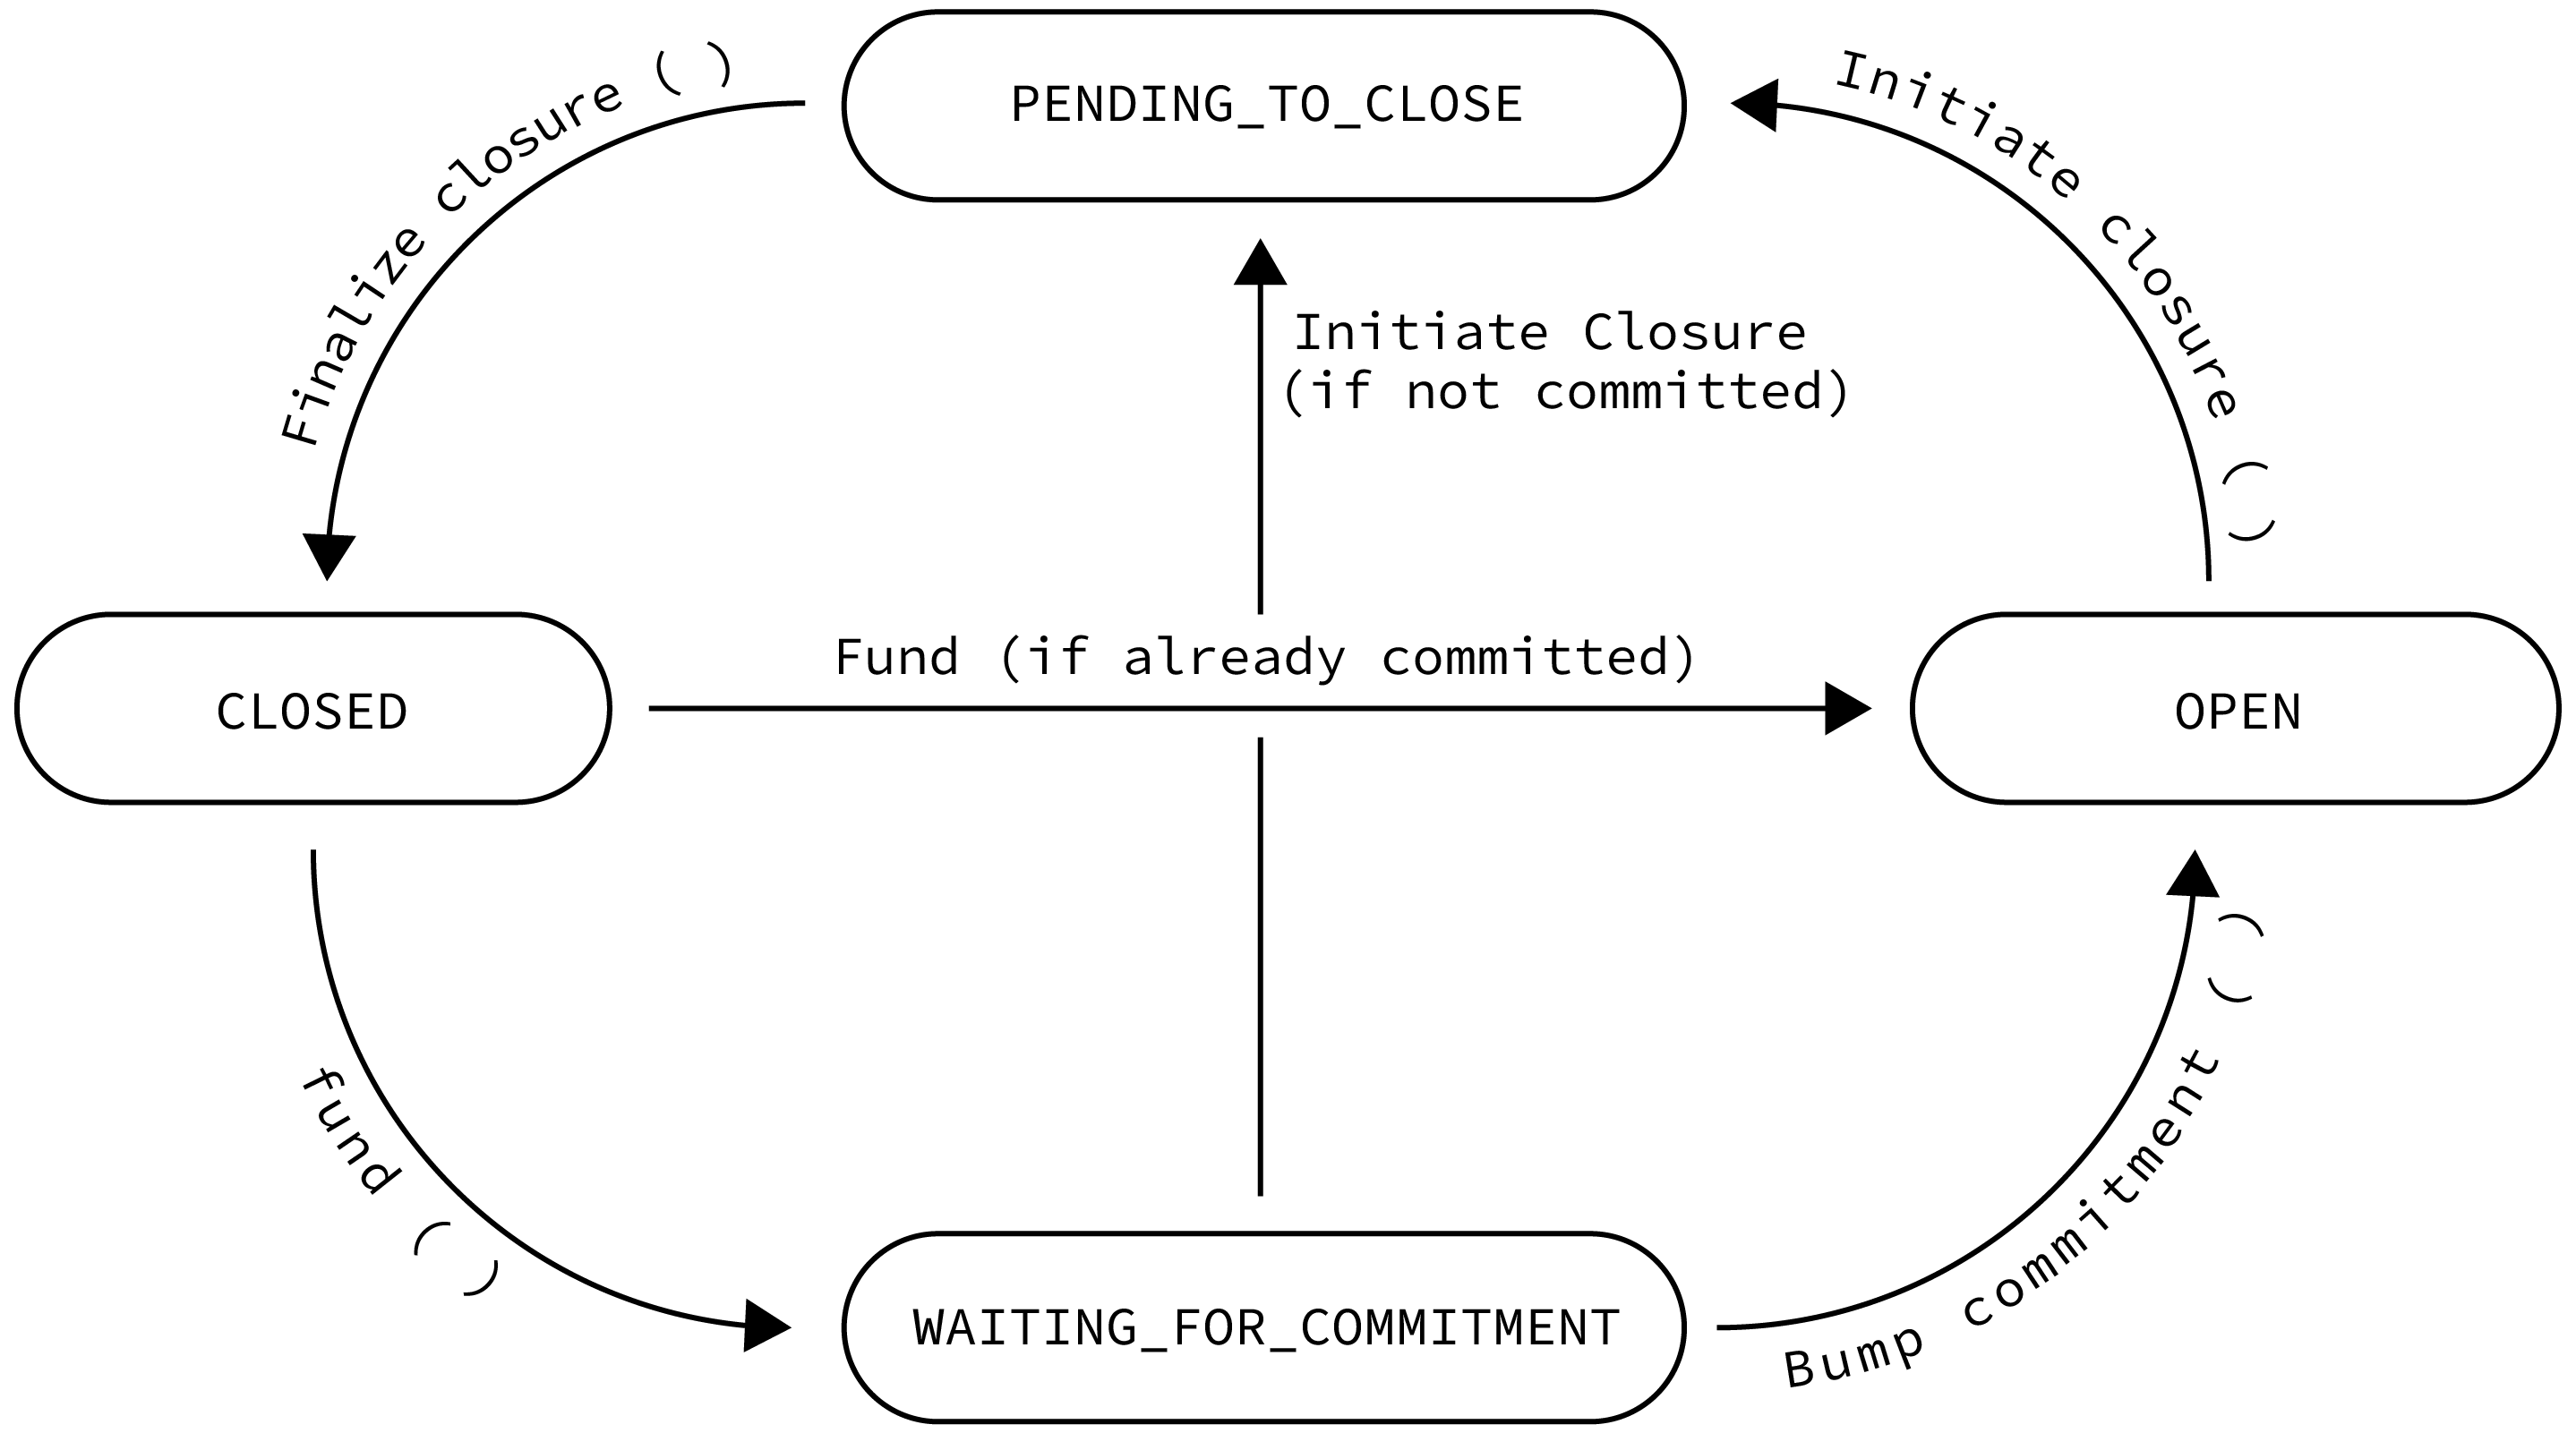
\includegraphics[width=9cm,height=9cm,keepaspectratio]{../yellowpaper/images/statesTransition.png}
    \label{fig:payment channel states}
    \caption{Payment channel states}
\end{figure}
Initially, each payment channel is \textit{Closed}. 

\paragraph{Opening a channel} Node $A$ can open a channel by transferring funds to the payment channels contract \textit{HoprChannels} and including the following \textit{userdata}:

$$[A: address, B: address, \lambda: uint8, \mu: uint8], \mu = 0,$$

where $\lambda$ is the amount to be staked by $A$. This call will trigger an on-chain event \textit{ChannelFunded} and open a unidirectional payment channel from $A$ to $B$. The payment channel will start in state \textit{Waiting for commitment}. The destination address of the payment channel must now set an on-chain commitment in order for the payment channel between both parties to become \textit{Open}. This is done by $B$ calling the \textit{bumpChannel()} function to make a new set of commitments towards this payment channel. This call will trigger an on-chain event \textit{ChannelOpened} and bumps the ticket epoch to ensure tickets with the previous epochs are invalidated. Every time the channel changes its state, an on-chain event \textit{ChannelUpdated} is emitted.

\paragraph{Redeeming tickets}
As long as the channel remains open, nodes can claim their incentives for forwarding packets via tickets. Tickets are redeemed by dispatching a \textit{redeemTicket()} call to an \textit{Open} payment channel.

If $B$ tries to redeem a ticket from the channel $A\rightarrow B$ (spending channel), but there is an open channel $B\rightarrow A$ (earning channel), $B$'s rewards will be transferred to $B\rightarrow A$ (earning channel). Otherwise, rewards will be sent directly to $B$.

\paragraph{Closing a channel}
Nodes can close a payment channel in order to access their previously staked funds. Only the payment channel creator can initiate the process by calling \textit{initiateChannelClosure()}. This changes the state to $Pending to close$ and triggers a grace period during which the destination node can redeem any unredeemed tickets. Nodes should actively monitor blockchain events to be aware of this payment channel state change.

Once the grace period has elapsed, the payment channel creator can call \textit{finalizeChannelClosure()} which changes the payment channel to $Closed$. When a payment channel is closed, the remaining funds are automatically transferred to the payment channel creator. The channel epoch increments, meaning any unredeemed tickets can no longer be redeemed.

\begin{comment}

\begin{figure}[H]
    \centering
    \begin{tikzpicture}[looseness=1,auto]
        \path (0,0) node (closed) [ellipse,draw] {$Closed$};
        \path (-1,-1)  node (commitment) [ellipse,draw,align=left] {$Waiting$\\$Commitment$};
        \path (5,0)  node (open) [ellipse,draw] {$Open$};
        \path (2.5,-1)  node (pending) [ellipse,draw,align=left] {$Pending$\\$Timeout$};

        \draw [->,draw](closed) to [bend left] node {\textsf{fund()}} (commitment);
        \draw [->,draw](commitment) to [bend left] node {\textsf{fund()}} (open);
        \draw [->,draw](open) to [bend left] node [align=center] {\textsf{initiateChannelClosure()}} (pending);
        \draw [->,draw](pending) to [bend left] node {\textsf{finalizeChannelClosure()}} (closed);

        \path[->] (open) edge [out=+120,in=+60,distance=2em,below] node [align=center,above] {\textsf{redeemTicket()}}  (open);
    \end{tikzpicture}
    \label{fig:channel workflow}
    \caption{Channel workflow}
\end{figure}
\end{comment}

\begin{comment}
  \draw [->,draw](commitment) to [bend left] node {\textsf{fund()}} (open);
    \draw [->,draw](open) to [bend left] node [align=center] {\textsf{initiateChannelClosure()}} (pending);
    \draw [->,draw](pending) to [bend left] node {\textsf{finalizeChannelClosure()}} (closed);  
\end{comment}

